\title{Digitales Theremin}

\team{%
    Andreas Frei,
    Dennis Aeschbacher}

\client{Hanspeter Schmid}

\coaches{%
    Hanspeter Schmid,
    Karl Schenk,
    Michael Pichler}

\fssummary{
Das Theremin kennen heutzutage nur wenige Leute, obwohl es das erste elektronische Instrument war. 
Dabei ist es einzigartig, da es ohne Berührung gespielt wird. Die Tonhöhe und Lautstärke kann über die Distanz zu zwei Antennen gesteuert werden. 
Jedoch kann dieses sonst rein analoge Instrument auch digital aufgebaut werden.
}

\fsgraphics{
	\centering

    \begin{minipage}{0.5\textwidth}
    	\centering
        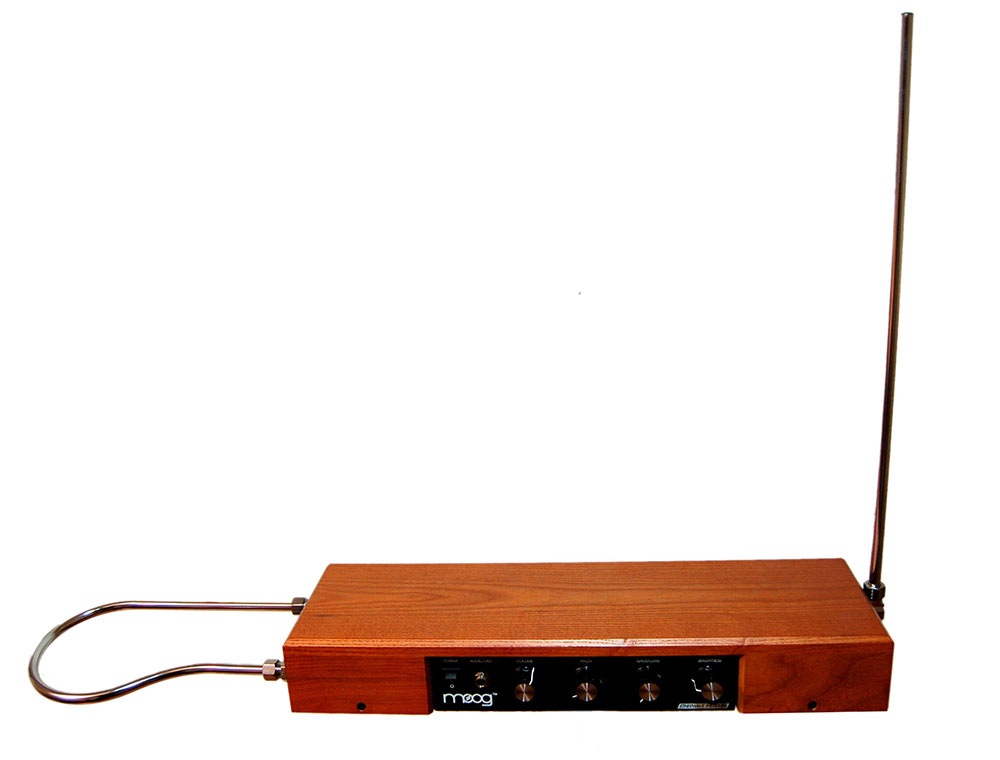
\includegraphics[width=\textwidth,height=65mm]{ThereminMoog}
        
        \graphicscaption{klassisches Theremin}
    \end{minipage}%
    \begin{minipage}{0.5\textwidth}
    	\centering
        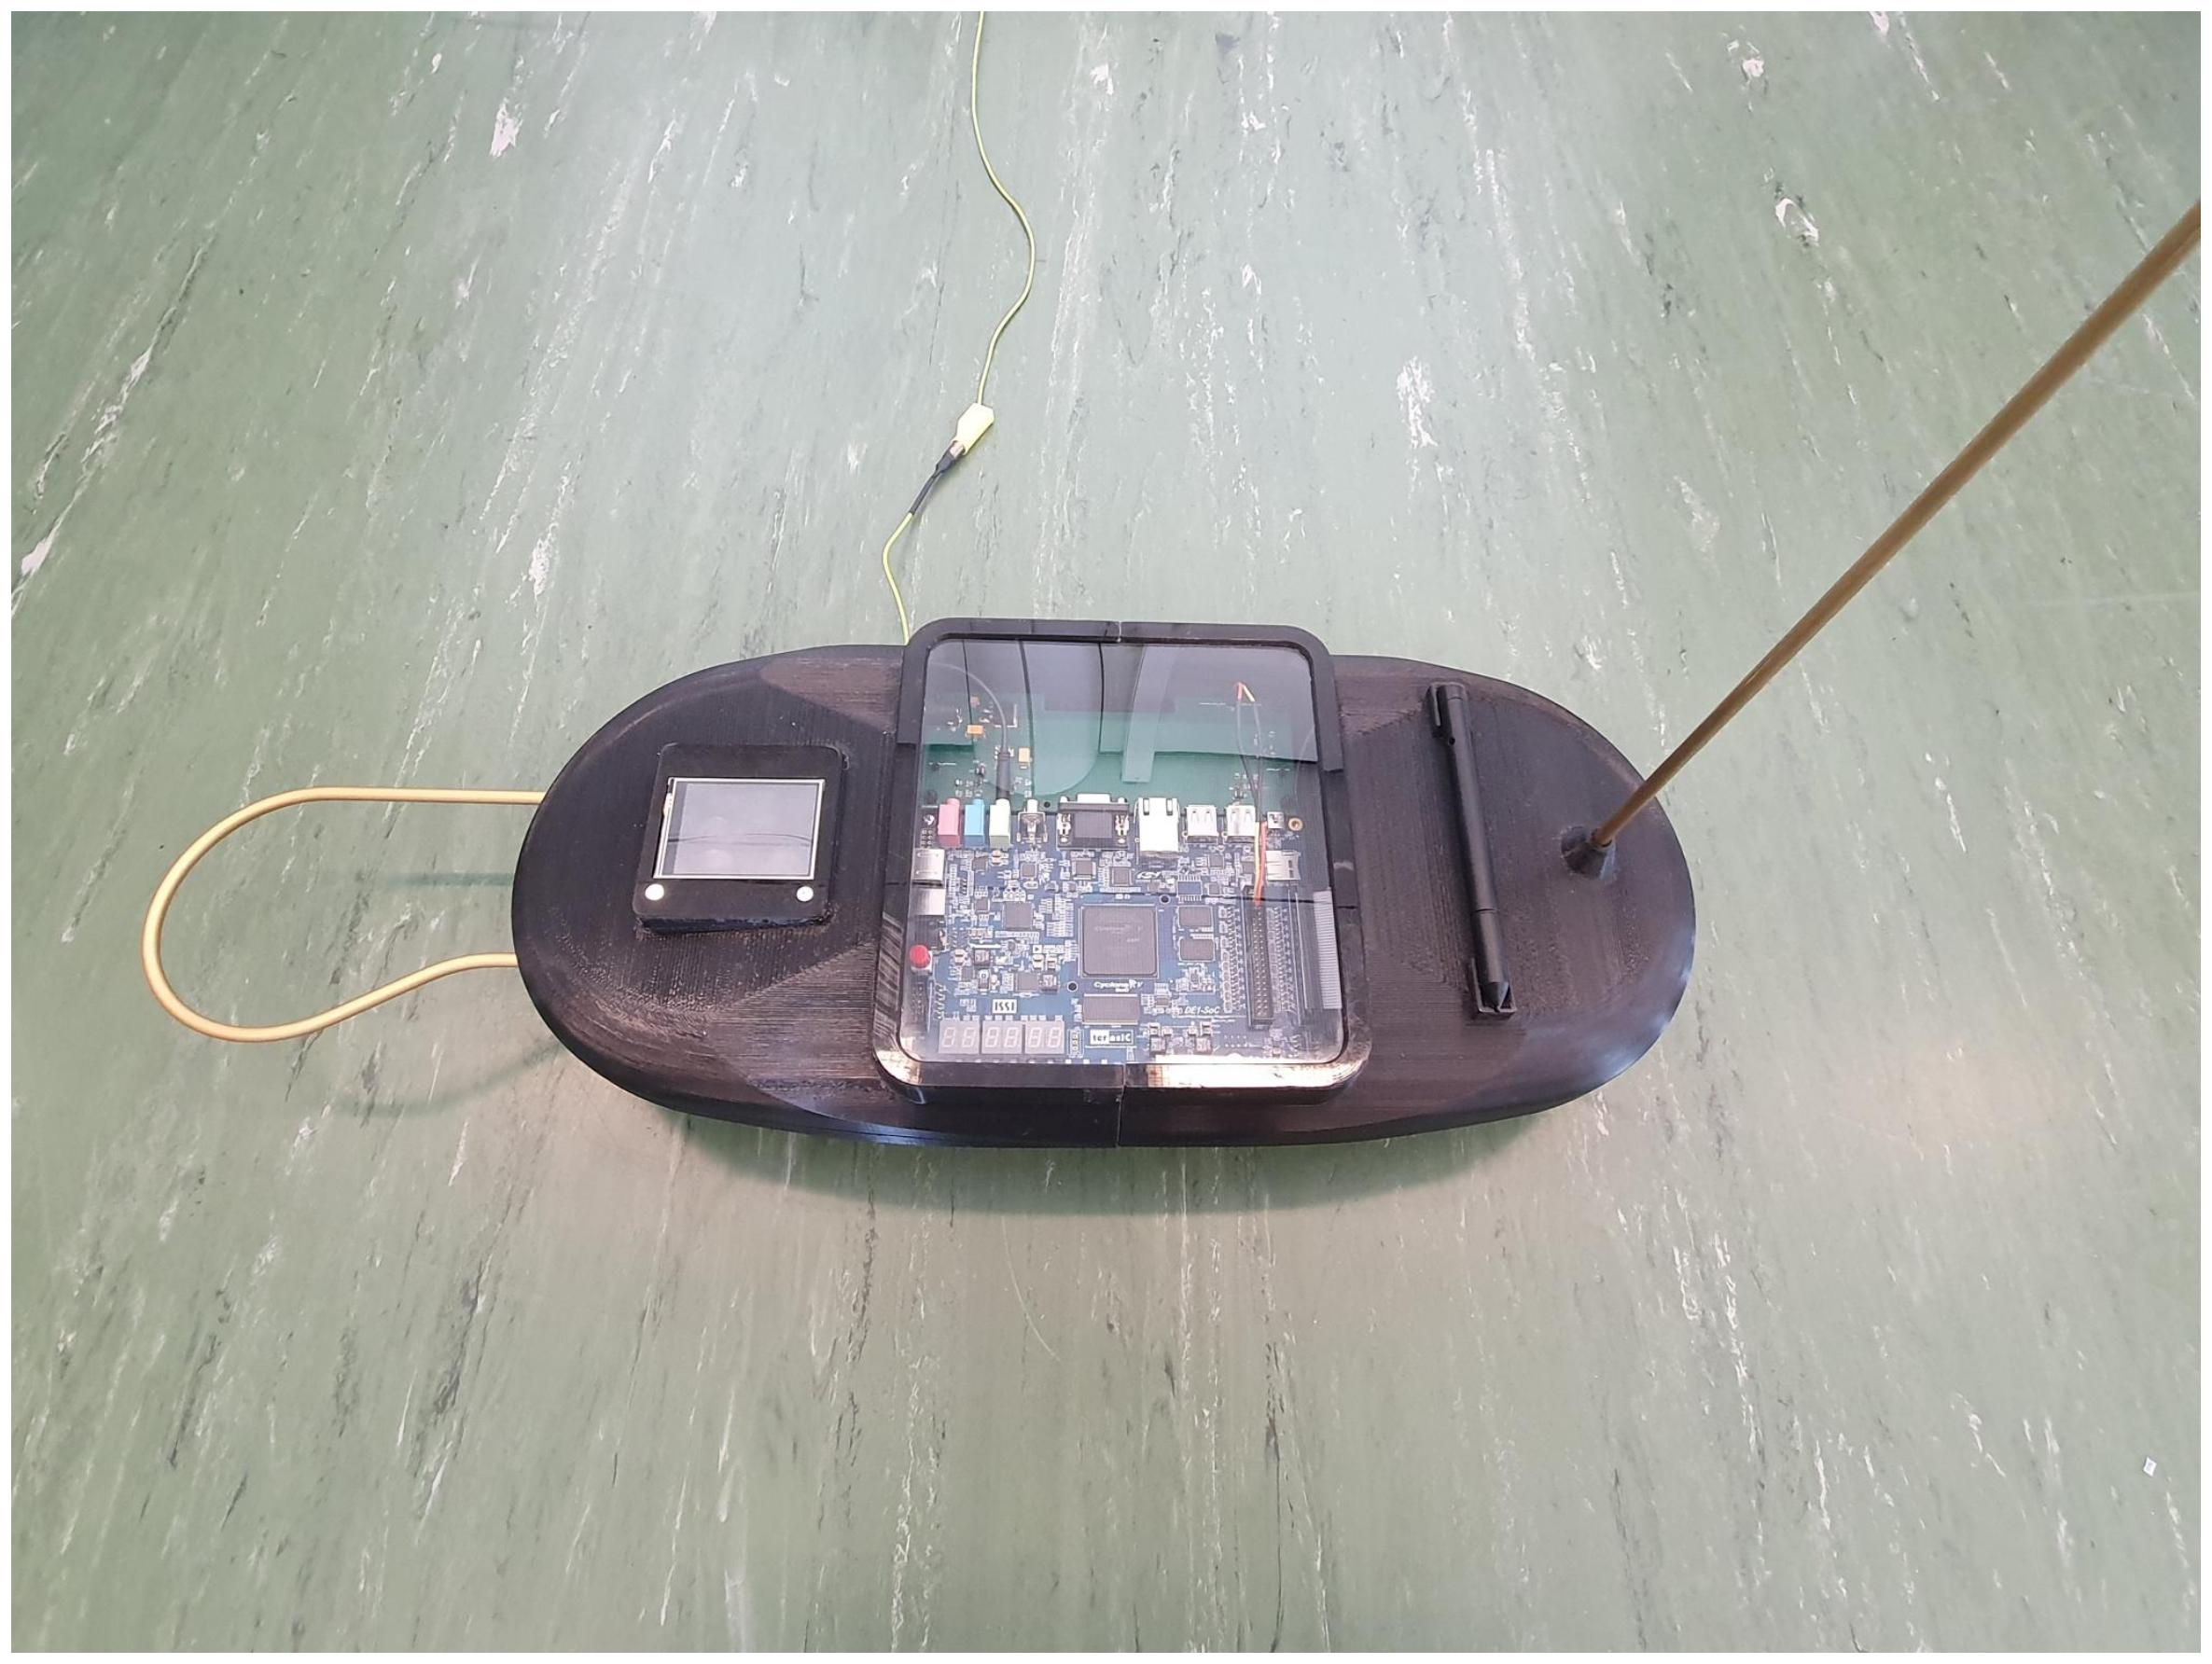
\includegraphics[width=\textwidth,width=90mm]{0001}
        
        \graphicscaption{digitales Theremin}
    \end{minipage}%
    
   
   
}

\fscontent{
    \section{Die Aufgabe}
	Immer mehr Geräte werden digital und dieser Trend scheint nicht abzuflachen. 
	Auch in diesem Projekt war es das Ziel, das sonst rein analoge Theremin digital aufzubauen.
	Des Weiteren soll es auf einem Field Programmable Gate Array (FPGA) aufgebaut werden. 
	Später soll es als Messeobjekt verwendet werden, um die Möglichkeiten dieser Technologie zu zeigen. 
	Um den Titel Messeobjekt zu verdienen soll es in ein ansprechendes Gehäuse verbaut und zusätzliche Effekte implementiert werden.
	
	
	

    \newcol
    \section{Die L\"osung}
    Um das Theremin weiter wie zuvor spielen zu können, wurden die Antennen weiter analog beibehalten. 
    Jedoch wurde die Signalverarbeitung für die Tonhöhe und Lautstärke auf dem DE1-SoC Board von terasIC aufgebaut. 
    Dabei wurden verschiedenste Verfahren verwendet um die Funktionsweise des Theremins auf eine digitale Signalverarbeitung zu übertragen.
	Das Theremin kann über einen Touchscreen bedient werden. Der implementierte Nios II Processor steuert dieses Display und die Signalverarbeitung. 
	Um das Theremin einfacher bedienen zu können wurden drei Zusatzfunktionen implementiert. Auf Knopfdruck kann das Theremin automatisch kalibriert werden, um einfacher die Töne zu treffen kann der Glissando-Effekt aktiviert werden und die Anzeige des gespielten Tons gibt dem Benutzer Feedback wie genau die Töne getroffen wurden.

    \newcol
    \section{Ausblick}
    Das Theremin kann nun gut in Messen als Ausstellungsobjekt eingesetzt werden und kann Besucher schon von weitem anlocken. Trotzdem hat es noch Verbesserungspotenzial. Ein Redesign des PCB könnte die letzten EMV und Aliasing Probleme lösen. Weiter könnten noch Zusatzeffekte implementiert werden wie Beispielsweise das Verändern des Sinus in eine Sägezahn- oder Dreiecksform um andere Instrumente anzunähern
}

\infobox{Jetztiger Stand}{%
   Das Theremin kann nun wie ein klassisches Theremin gespielt werden, nachdem zusätzlich die Lautstärkenverarbeitung implementiert wurde. Der spielbare Bereich geht von etwa 100Hz bis ca. 2kHz. Weiter hat das Theremin drei Zusatzfunktionen: Es kann automatisch Kalibriert werden, Es hat eine Funktion, welches dem Benutzer hilft richtige Töne zu treffen und kann dem Spieler Feedback geben, wie genau er am Spielen ist.
}
